\documentclass{beamer}
\usepackage{beamerthemeshadow}
\usepackage{verbatim}
\usepackage{array}

\usepackage{lastpage}
\usepackage{xcolor}
\usepackage{pgf}
\usepackage{colortbl}
\usepackage{hyperref}
\usepackage{multirow}

\usepackage{siunitx}
\sisetup{input-symbols=(), group-digits  = false} 

\newcommand{\bi}{\begin{itemize}}
\newcommand{\ei}{\end{itemize}}
\newcommand{\be}{\begin{enumerate}}
\newcommand{\ee}{\end{enumerate}}
\newcommand{\bd}{\begin{description}}
\newcommand{\ed}{\end{description}}
\newcommand{\prbf}[1]{\textbf{#1}}
\newcommand{\prit}[1]{\textit{#1}}
\newcommand{\beq}{\begin{equation}}
\newcommand{\eeq}{\end{equation}}
\newcommand{\bdm}{\begin{displaymath}}
\newcommand{\edm}{\end{displaymath}}

\newcommand{\ft}[1]{
  \frametitle{\begin{tabular}{p{4.2in}r} \textcolor{white}{#1} & \small{\insertframenumber / \inserttotalframenumber} \end{tabular}}
  \setbeamercovered{transparent=18}
}

\newcommand{\eft}[1]{
  \frametitle{\begin{tabular}{p{4in}r} \textcolor{white}{#1} & \small{\hyperlink{f:questions}{\beamergotobutton{GO BACK}}} \end{tabular}}
  \setbeamercovered{transparent=18}
}

\newcommand{\stepinv}{\setbeamercovered{invisible}}
\newcommand{\stopinv}{\setbeamercovered{transparent=18}}
\newcommand{\uncoverinv}[1]
{
  \setbeamercovered{invisible}
  \uncover<+->{#1}
  \setbeamercovered{transparent=18}
}
\newcommand{\ans}[1]{\textcolor{blue}{#1}}
\newcommand{\ansinv}[1]
{
  \setbeamercovered{invisible}
  \uncover<+->{\textcolor{blue}{#1}}
  \setbeamercovered{transparent=18}
}
\newcommand{\setinv}{\setbeamercovered{invisible}}
\newcommand{\setvis}{\setbeamercovered{transparent=18}}
\newcommand{\centerpic}[2]
{
  \begin{center}
  \includegraphics[#1]{#2}
  \end{center}
}
\newcommand{\h}[1]{\hat{#1}}
\newcommand{\ds}{\displaystyle}

\definecolor{light}{rgb}{0,0.75,0.85}
\definecolor{BrickRed}{rgb}{0.0,0.1,0.4}
\newcommand{\hl}[1]{\only<#1>{\cellcolor{light}}}

\definecolor{mycolor}{rgb}{0.0,0.5,0.8}
\usecolortheme[named=mycolor]{structure}

\title[Fiscal Policy Uncertainty and Macroeconomic Consequences]{Fiscal Policy Uncertainty and Its Macroeconomic Consequences}
\author[James Murray, University of Wisconsin - La Crosse]
{
James Murray\\
Department of Economics\\
University of Wisconsin - La Crosse
}
\date{MEA 2015 Annual Meeting\\Minneapolis, MN\\~\\March 28, 2015}

\begin{document}

\frame{\titlepage \setcounter{framenumber}{0}}

\frame
{
  \ft{Purpose 1: Quantify Fiscal Uncertainty}
  \begin{block}{Existing Contributions}
    \bi
    \item Time-varying volatility of a DSGE fiscal shock:\\
      ~~~Fern\'andez-Villiverde et. al. (2011), Born and Pfeifer (2011).
    \item Index based on newspaper headlines and other real world stuff:\\
      ~~~Baker et. al. (2013)
    \ei
  \end{block}

  \begin{block}{Present Paper}
      \bi
      \item Every period, agents estimate regressions describing fiscal policy behavior.
      \item Not unlike early sections of Fern\'andez-Villiverde et. al. (2011), Born and Pfeifer (2011).
      \item Forecast uncertainty:  Fiscal policy uncertainty should be related to the variance of forecasts.
      \ei
  \end{block}
}

\frame
{
  \ft{Purpose 2: Estimate Macroeconomic Consequences}
  \begin{block}{Fiscal Policy Variables}
    \begin{columns}
    \begin{column}{0.4\textwidth}
    \be
    \item Government Spending
    \item Tax Revenue
    \item Net Transfers
    \item Government Debt
    \ee
    \end{column}

    \begin{column}{0.5\textwidth}
        \bi
        \item \textit{Construct an uncertainty measure for each.}
        \item \textit{Construct an index for overall fiscal uncertainty}
        \ei
    \end{column}
    \end{columns}
  \end{block}

  \begin{block}{Impact on Macroeconomy}
  Incorporate measures of fiscal uncertainty in ARDL models for:
    \be
    \item Consumption
    \item Investment
    \item Real GDP
    \item Employment
    \item Unemployment
    \item Inflation
    \ee  
  \end{block}
}

\begin{comment}
\frame
{
  \ft{Literature}
  \begin{block}{Time-varying Fiscal Volatility}
  \bi
  \item Fern\'andez-Villiverde et. al. (2011a): Fiscal policy uncertainty is stagflationary
  \item Born and Pfeifer (2011): Not a significant driver for business cycles.
  \item Johannsen (2012): Matters more at ZLB.
  \ei
  \end{block}

  \begin{block}{Other Constructions for Fiscal Uncertainty}
  \bi
  \item Baker (2013): Uncertainty reduces economic activity
  \item Hollmayr and Matthes (2013): Bayesian learning for switching fiscal behavior
    \bi
    \item Permanent fiscal changes can have a small economic impact
    \item Learning increases macroeconomic volatility
    \ei
  \ei
  \end{block}

}


\frame
{
  \ft{Literature}

  \begin{block}{Forward Looking Fiscal Uncertainty}
    \bi
    \item Bi, Leith, and Leeper (2013): Timing and composition of fiscal contractions
    \item Davig, Leeper, and Walker (2010):  Uncertain future for unfunded entitlement programs is stagflationary
    \item Davig and Foerster (2014): Possibly expiring tax provisions decrease investment and employment
    \item Richter and Throckmorton (2014): Uncertain debt targets possibly welfare enhancing or reducing
    \ei
  \end{block}
  
}
\end{comment}

\frame
{
  \ft{Spoiler}
  Fiscal Uncertainty Reduces Economic Activity

  \bi
  \item General measure for fiscal uncertainty associated with:
    \bi
    \item lower real GDP,
    \item lower consumption,
    \item lower investment.
    \ei
 
  \item Uncertainty regarding specific fiscal variables 
    \bi
    \item Government expenditures, transfer payments, and government debt associated with reductions in employment / increases in unemployment
    \item Tax uncertainty associated with increases in investment and real GDP
    \ei

  \item General fiscal uncertainty significant drag during the Great Recession:
    \bi
    \item Responsible for a 1\% to 3\% decrease in real GDP
    \item Decreased consumption by about 1\% of real GDP
    \item Decreased investment by about 1\% of real GDP
    \ei
  \ei
}

\frame
{
  \ft{Constant Gain Learning}
  \begin{block}{Constant gain learning mechanism}
    \bi
    \item Every period, run a least-squares regression for each fiscal policy variable, using data from previous periods.
    \item Weighted least squares - more recent observations have more weight.
    \item Regression predicted value serves as expected fiscal policy.
    \item Root (weighted) mean squared error serves as \textit{fiscal policy uncertainty}.
    \ei
  \end{block}

 \begin{block}{Ideal situations for constant gain learning}
    \bi
    \item Precedence of structural changes
    \item No a-priori knowledge on menu or evolution of structural changes and probability distributions
    \item Forecasting rule, but no knowledge of parameter values, or the structure of the whole economy.
    \ei
  \end{block}

}

\frame
{
  \ft{Fiscal Policy Regressions}
  \begin{block}{Four regressions}
  \textbf{Fiscal policy variables:} $f_{t} = [g_t~ r_t~ n_t~ b_t]$ \\ 
  Govt Spending ($g_t$), Tax Revenue ($r_t$),\\
  Net Transfers ($n_t$), Government Debt / GDP ($b_t$) \\ [0.5pc]

  \textbf{Regression equation:}\\
  $f_{i,t} = \alpha_{t,0} + \alpha_{t,f}' f_{t-1} + \alpha_{t,y} y_{t} + \alpha_{t,c} c_t + \alpha_{I,t} I_t + \alpha_{t,u} u_{t} + \epsilon_t$
  \end{block}

  \begin{block}{Empirical Model for Fiscal Policy Behavior}
  Each fiscal policy variable ($f_{i,t}$) responds to:
  \bi
  \item Lag of all fiscal policy variables ($f_{t-1}$).
  \item Above includes lag of government debt ($b_{t-1}$).
  \item Macro outcomes: real GDP ($y_t$), consumption ($c_t$), investment ($I_t$), and unemployment ($u_t$).
  \item All quantities real, per capita, ratio of past real GDP.
  \ei
  \end{block}
}

\frame
{
  \ft{Least-Squares Learning}
  \begin{block}{Understanding Fiscal Policy}
    \bdm \hat{\alpha}_t = \left(\sum_{\tau=0}^{t} w_{\tau} X_{\tau} X_{\tau}' \right)^{-1} \left(\sum_{\tau=0}^{t} w_{\tau} X_{\tau}' f_{i,\tau} \right) \edm
    \bi
    \item Time $t$ expected fiscal action: $E_t^* f_{i,t} = X_t' \hat{\alpha}_{t-1}$
    \item Information set includes \textit{past fiscal behavior} and \textit{current macro conditions}.
    \item Unexplained policy: $\hat{\epsilon}_t = f_{i,t} - X_t' \hat{\alpha}_{t-1}$
    \ei
  \end{block}

  \begin{block}{Constant Gain Learning}
    \bi
    \item Weight on $t-\tau$ observation: $\omega_\tau = (1-\gamma) \gamma^{\tau}$.
    \item \textbf{Learning gain}, $\gamma \in (0,1)$, is constant weight assigned to most recent observation.
    \item $\gamma \approx 0.02$ (Milani (2008), Slobodyan and Wouters (2008)).
    \ei
  \end{block}
}


\frame
{
  \ft{Instrumental Variable Learning} 
  \begin{block}{Endogeneity Problem}
  \bi 
  \item Macro outcomes (real GDP, consumption, investment, and unemployment) are likely endogenous.
  \item Use instruments: lags of macro outcomes and fiscal variables
  \item Two-stage least squares - using constant gain weighting procedure above.
  \ei
  \end{block}

  \begin{block}{Fiscal Uncertainty}
  Unexplained fiscal policy: $\epsilon_{i,t} = f_{i,t} - \hat{\alpha}_{i,t-1}^{IV'} X_t$\\
  Fiscal Uncertainty given by Root (weighted) mean squared error:\\
    \bdm m_{i,t}^{IV} = \sqrt{ (1-\gamma) \ds \sum_{\tau=1}^{t} \gamma^{\tau} \epsilon_{i,t}^2} \edm
  \end{block}
}

\frame
{
  \ft{Fiscal Policy - Actual and Predicted}
  \begin{tabular}{cc}
    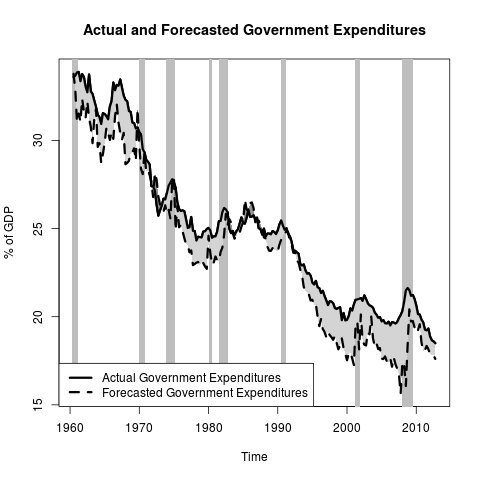
\includegraphics[width=0.45\textwidth, height=0.45\textheight]{pics/pred_gov.png} & 
    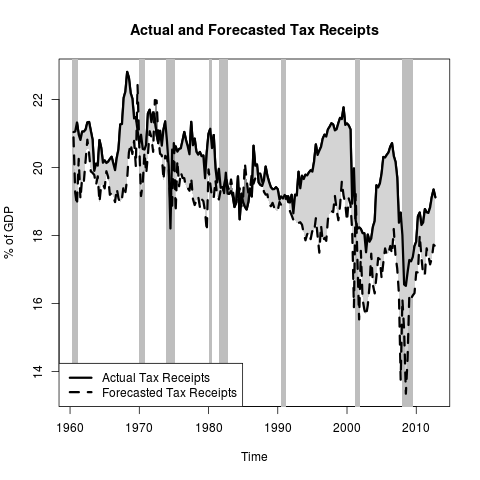
\includegraphics[width=0.45\textwidth, height=0.45\textheight]{pics/pred_tax.png} \\ 
    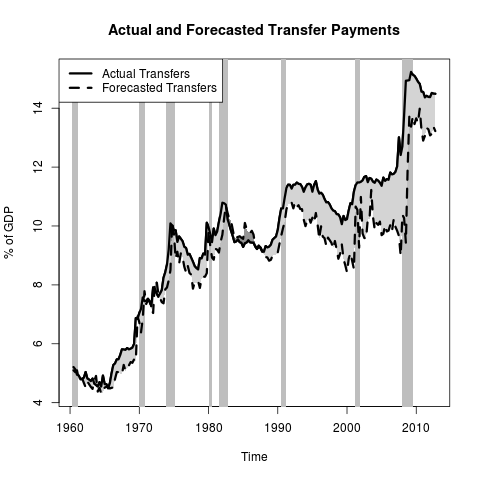
\includegraphics[width=0.45\textwidth, height=0.45\textheight]{pics/pred_transfers.png} & 
    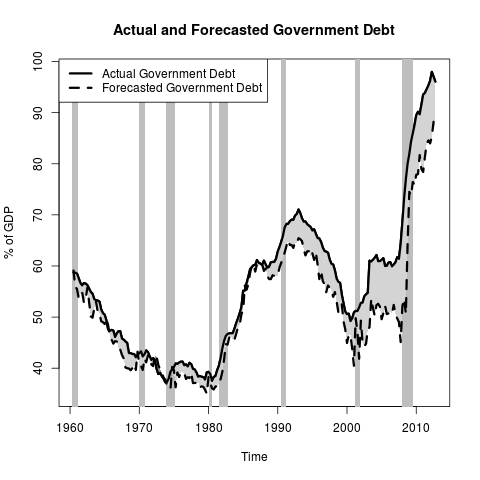
\includegraphics[width=0.45\textwidth, height=0.45\textheight]{pics/pred_debt.png} 
  \end{tabular}
}

\frame
{
  \ft{Fiscal Policy Uncertainty}
  \begin{tabular}{cc}
    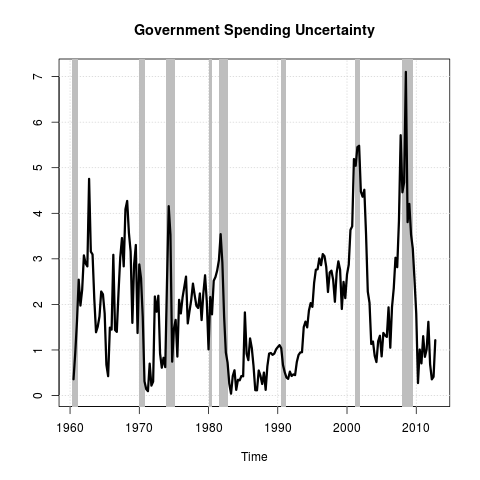
\includegraphics[width=0.45\textwidth, height=0.45\textheight]{pics/fpu_gov.png} & 
    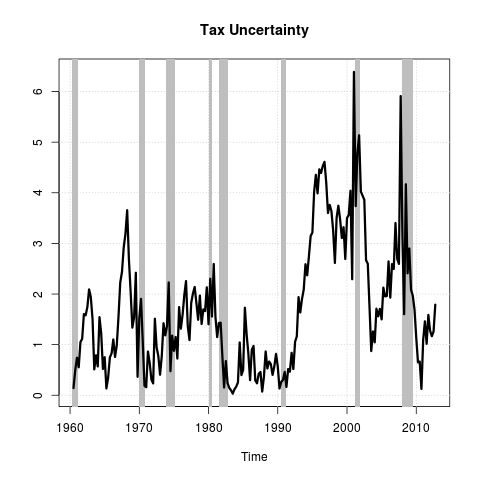
\includegraphics[width=0.45\textwidth, height=0.45\textheight]{pics/fpu_tax.png} \\ 
    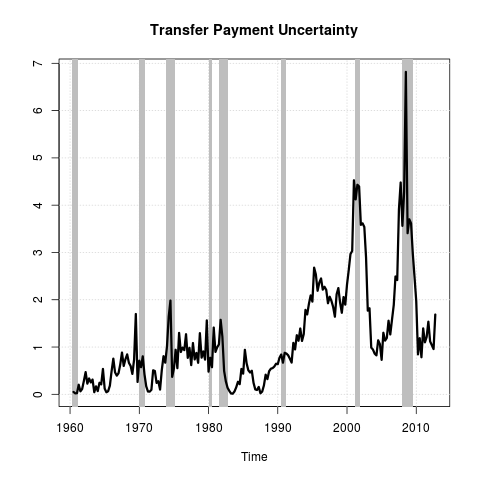
\includegraphics[width=0.45\textwidth, height=0.45\textheight]{pics/fpu_transfers.png} & 
    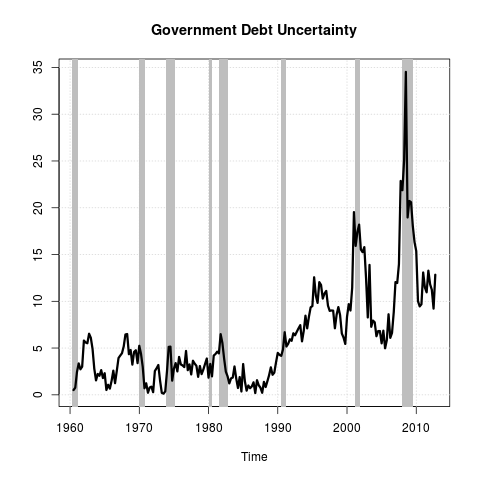
\includegraphics[width=0.45\textwidth, height=0.45\textheight]{pics/fpu_debt.png} 
  \end{tabular}
}

\frame
{
  \ft{Casual Observations}
  \bi
  \item Uncertainty concerning transfers and debt reached unprecedented levels during Great Recession.
    \bi
    \item Government expenditures uncertainty: Nearly 7\% of GDP
    \item Tax uncertainty: Nearly 6\% of GDP
    \item Transfers uncertainty: Nearly 7\% of GDP
    \item Government debt uncertainty: Nearly 35\% of GDP
    \ei
  \item Uncertainty seems to run up for several years preceding recessions:
    \bi
    \item Early 1980s, 2001, 2007.
    \item Not the rule though (eg: declines prior to 1970s, little volatility prior to 1991)
    \ei
  \ei
}

\frame
{
  \ft{Fiscal Uncertainty Correlations}
\begin{scriptsize}
\begin{center}
\textbf{Pearson Correlation Coefficient} \\ \ \\
\begin{tabular}{l|cccc}
 & Gov Spending & Tax Revenue & Transfers & Government Debt \\ \hline
Gov Spending & 1.00 & - & - & - \\
Tax Revenue & 0.75 & 1.00 & - & - \\
Transfers & 0.74 & 0.78 & 1.00 & - \\
Government Debt & 0.64 & 0.65 & 0.90 & 1.00 \\ \hline
\end{tabular}
\end{center}
\end{scriptsize}
\bi
\item All highly correlated. 
\item Common (latent) factor?
\ei
}

\frame
{
  \ft{Fiscal Uncertainty Coincident Indicator}
  \begin{block}{Objective}
    \bi 
    \item Strip out the common component of fiscal uncertainty
    \item Construct a general measure of fiscal uncertainty
    \item Take care of potential multicolinearity problem
    \item Compare to Baker, Bloom, and Davis (2013) (BBD)
    \ei
  \end{block}    

  \begin{block}{Stock and Waston (1989) coincident indicator model}
  \bi
  \item Latent variable: General fiscal uncertainty
    
    \vspace*{-0.5pc} \bdm \begin{array}{l} m_t = m_0 + A \lambda_t + e_t \\ [0.2pc]
\lambda_t = b_1 \lambda_{t-1} + b_2 \lambda_{t-2} + \upsilon_t\\ [0.2pc]
e_t = C e_{t-1} + \eta_t \end{array} \edm
     \vspace*{-0.5pc} \bi
     \item $m_t$: 4x1 vector of fiscal uncertainty variables
     \item $\lambda_t$: general fiscal uncertainty
     \item $m_0 + e_t$: idiosyncratic component of fiscal uncertainty.
     \ei
   \ei
   \end{block}
}

\frame
{
  \ft{Coincident Indicator: General Fiscal Uncertainty}
  \begin{center}
    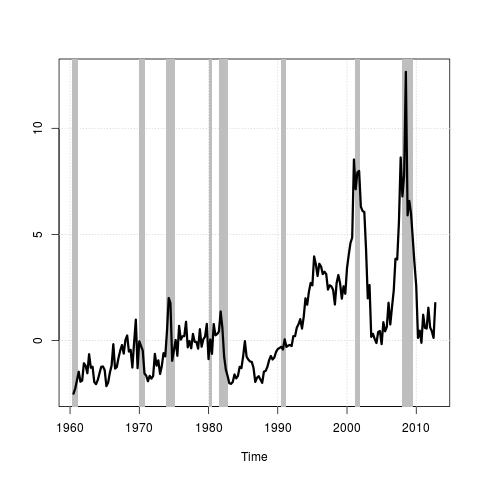
\includegraphics[width=0.8\textwidth]{pics/fpucoin.png}
  \end{center}
}

\begin{comment}
\frame
{
  \ft{Idiosyncratic Fiscal Uncertainty}
  \begin{tabular}{cc}
    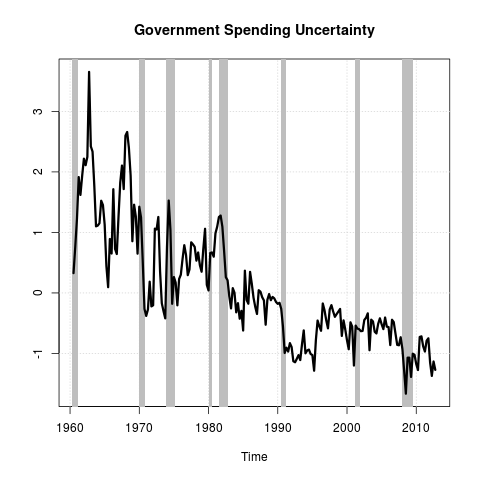
\includegraphics[width=0.45\textwidth, height=0.45\textheight]{pics/fpucoin_gov.png} & 
    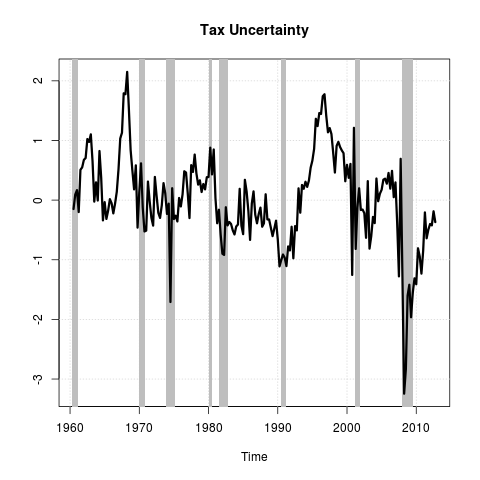
\includegraphics[width=0.45\textwidth, height=0.45\textheight]{pics/fpucoin_tax.png} \\ 
    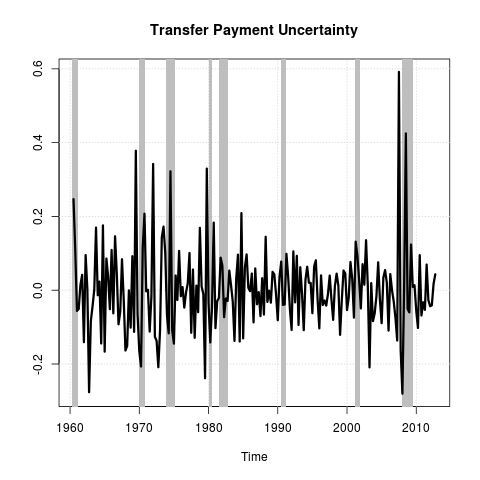
\includegraphics[width=0.45\textwidth, height=0.45\textheight]{pics/fpucoin_transfers.png} & 
    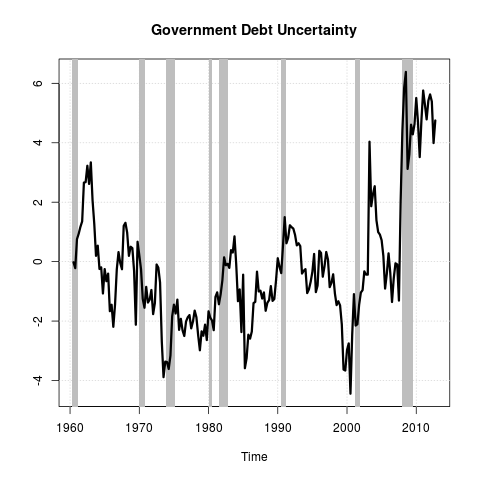
\includegraphics[width=0.45\textwidth, height=0.45\textheight]{pics/fpucoin_debt.png} 
  \end{tabular}
}
\end{comment}

\frame
{
  \ft{Fiscal Uncertainty Correlations Redux}
\begin{scriptsize}
\begin{center}
\textbf{Idiosyncratic Fiscal Uncertainty - Pearson Correlations}\\ \ \\
\begin{tabular}{l|cccc}
 & Gov Spending & Tax Revenue & Transfers & Government Debt \\ \hline
Gov Spending & 1.00 & - & - & - \\
Tax Revenue & 0.40 & 1.00 & - & - \\
Transfers & -0.17 & -0.23 & 1.00 & - \\
Government Debt & -0.21 & -0.32 & -0.18 & 1.00 \\ \hline
\end{tabular}
\end{center}
\end{scriptsize}
\ \\ \ \\

\begin{scriptsize}
\begin{center}
\textbf{Correlation of RMSE with Coincident Index}\\ \ \\
\begin{tabular}{l|cccc}
 & Gov Spending & Tax Revenue & Transfers & Government Debt \\ \hline
Coincident Index~ & 0.75 & 0.78 & 0.99 & 0.91 \\ \hline
\end{tabular}
\end{center}
\end{scriptsize}
}

\frame
{
  \ft{Relationship with Baker et. al. (2013)}
\begin{footnotesize}
\hspace*{-2pc}\begin{tabular}{ccc}
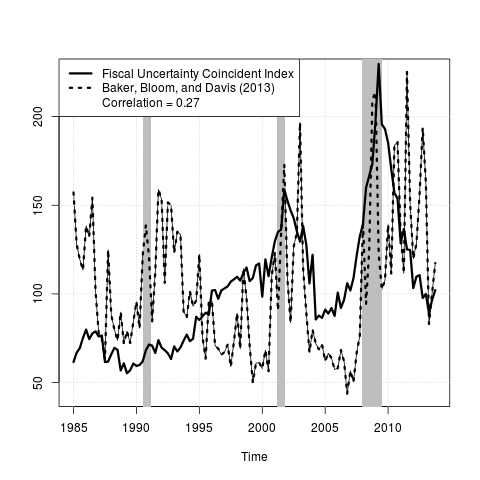
\includegraphics[scale=0.22]{./results/pics0.01/fpuindex.png} & 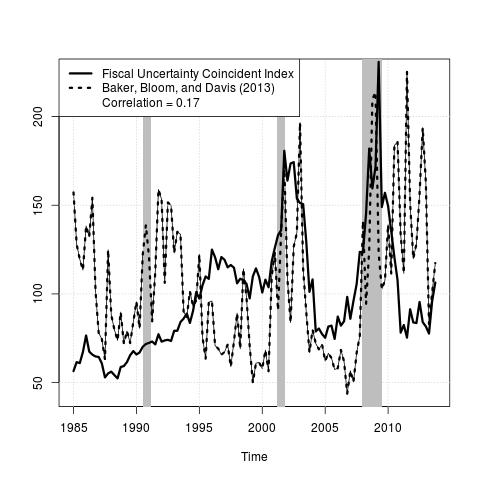
\includegraphics[scale=0.22]{./results/pics0.02/fpuindex.png} & 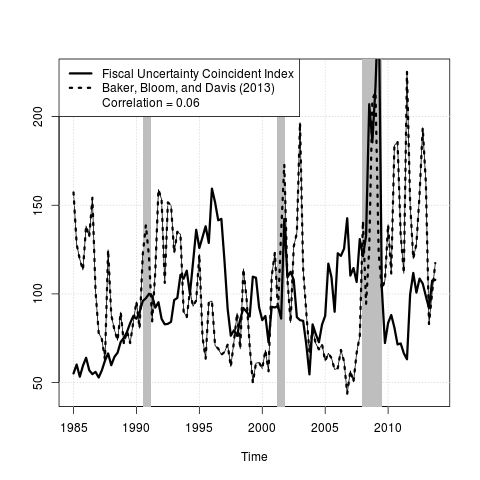
\includegraphics[scale=0.22]{./results/pics0.04/fpuindex.png} \\
Learning Gain = 0.01 & Learning Gain = 0.02 & Learning Gain = 0.04  \\
Correlation = 0.27 & Correlation = 0.17 & Correlation = 0.06 \\
\end{tabular}
\bi
\item Close match post-2000
\item Higher correlation with more empirically plausible learning gains
\item BBD - Headline news is likely endogenous
\item BBD - Tax policy expiration is forward looking
\item BBD is a general economic policy uncertainty index
\ei
\end{footnotesize}
}

\frame
{
  \ft{Autoregressive Distributed Lag Model}
  %\begin{footnotesize}
  \begin{block}{Dependent Variables: Macroeconomic Outcomes}
    \vspace*{-0.5pc}\begin{columns}
      \column{0.3\textwidth}
      \bi \item Real GDP \item Consumption  \ei
      \column{0.3\textwidth}
      \bi \item Investment \item Inflation \ei 
      \column{0.3\textwidth}
      \bi \item Employment \item Unemployment \ei
      \column{0.05\textwidth}~
    \end{columns}
  \end{block}

  \begin{block}{Explanatory Vars: Common and Idiosyncratic Fiscal Uncertainty}
      \vspace*{-0.5pc}\begin{columns}[t]
      \column{0.4\textwidth}
      \bi \item Government Exp  \item Tax Receipts  \item Transfer Payments  \ei
      \column{0.55\textwidth}
      \bi \item Government Debt  \item Coincident Index \ei ~~~(First lag to avoid endogeneity)
      \column{0.05\textwidth}~
    \end{columns}
  \end{block}

  \begin{block}{Controls}
    \bi 
    \item Lags of all the dependent variables in every model.
    \item Lags of all the fiscal policy variables
    \ei
  \end{block}

  %\end{footnotesize}
}

\frame
{
  \ft{ARDL Results (Learning Gain = 0.02, Lags = 2)}

\begin{tiny}
\begin{center}
\begin{tabular}{l|S[table-format=3.2] S[table-format=3.2] S[table-format=3.2] S[table-format=3.2] S[table-format=3.2] S[table-format=3.2]}
\textbf{Fiscal Uncertainty} & \multicolumn{6}{c}{\textbf{Dependent Variables (Column Headings)}} \\
\textbf{ - Row Headings -}                 & \multicolumn{1}{p{0.4in}}{\vspace*{-1.5pc}\begin{center}~\newline Real GDP\end{center}} 
                & \multicolumn{1}{p{0.4in}}{\vspace*{-1.5pc}\begin{center}Consumption\end{center}} 
                & \multicolumn{1}{p{0.4in}}{\vspace*{-1.5pc}\begin{center}~\newline Investment\end{center}} 
                & \multicolumn{1}{p{0.4in}}{\vspace*{-1.5pc}\begin{center}Employment\end{center}}
                & \multicolumn{1}{p{0.4in}}{\vspace*{-1.5pc}\begin{center}Unemployment\end{center}} 
                & \multicolumn{1}{p{0.4in}}{\vspace*{-1.5pc}\begin{center}~\newline Inflation\end{center}} \\ [-0.5pc] \hline
 & \multicolumn{6}{c}{} \\ [-0.25pc]
 Government Exp \hl{4} & -0.04 & 0.06 & -0.06 & -0.68** \hl{4} & 0.55*** \hl{4} & 0.02 \\
 (Standard Error) \hl{4} & (0.11) & (0.07) & (0.08) & (0.28) \hl{4} & (0.13) \hl{4} & (0.25) \\ [0.2pc]
 Tax Receipts \hl{6} & 0.36*** \hl{6} & 0.07  & 0.26*** \hl{6} & 0.39 & -0.22 & 0.05 \\
 (Standard Error) \hl{6} & (0.11) \hl{6} & (0.06) & (0.09) \hl{6} & (0.28) & (0.14) & (0.15) \\ [0.2pc]
 Transfer Payments \hl{4} & -0.01 & -0.03 & 0.01 & -0.49** \hl{4} & 0.19*** \hl{4}  & 0.01 \\
 (Standard Error) \hl{4} & (0.08) & (0.04) & (0.04) & (0.23) \hl{4}  & (0.06) \hl{4} & (0.12) \\ [0.2pc]
 Government Debt \hl{5}  & 0.05 & -0.03 & 0.09 & -1.27 \hl{5} & 0.25 \hl{5} & 0.12 \\
 (Standard Error) \hl{5}  & (0.10) & (0.06) & (0.06) & (0.88) \hl{5} & (0.16) \hl{5} & (0.17)  \\ [0.2pc]
 Coincident Index \hl{3} & -0.41*** \hl{3} & -0.21*** \hl{3} & -0.19*** \hl{3} & 0.13 & -0.22* & -0.36** \hl{3} \\
 (Standard Error) \hl{3} & (0.10) \hl{3} & (0.05) \hl{3} & (0.07) \hl{3} & (0.38) & (0.14) & (0.16) \hl{3} \\ [0.2pc]
\hline
 ~ \hl{2} & \multicolumn{6}{c}{ ~ \hl{2}} \\ [-0.25pc]
Joint Wald \hl{2} &  4.02*** \hl{2} &  3.80*** \hl{2} & 2.54** \hl{2} & 3.21*** \hl{2} & 4.27*** \hl{2} &  1.29 \hl{2} \\ [0.25pc] \hline

 & \multicolumn{6}{c}{} \\ [-0.25pc]
 Adjusted R-square & 0.32 & 0.98 & 0.96 & 0.83 & 0.87 & 0.81 \\
 AIC & 466.15 & 198.35 & 257.72 & 666.99 & 398.54 & 632.69 \\
 BIC & 549.83 & 282.03 & 341.40 & 750.67 & 482.22 & 716.37 \\ \hline

\end{tabular}

\end{center}
\end{tiny}
\begin{scriptsize}
\only<1>{~ \\  ~ \\ }
\only<2>{\textcolor{BrickRed}{\textbf{1. Fiscal uncertainty influences everything but inflation}}}
\only<3>{\textcolor{BrickRed}{\textbf{2. Common fiscal uncertainty dampens aggregate demand}}}
\only<4>{\textcolor{BrickRed}{\textbf{3. Transfers and Spending uncertainty drags on employment}}}
\only<5>{\textcolor{BrickRed}{\textbf{4. Debt uncertainty drags on employment (significant in most other specifications)}}}
\only<6>{\textcolor{BrickRed}{\textbf{5. Tax uncertainty (mostly unexpectedly low) boosts investment and real GDP}}}
\end{scriptsize}
}

\frame
{
  \ft{Impact from an Historical Buildup}
\begin{scriptsize}
\begin{center}
\textbf{Magnitude of Extreme Change in Coincident Fiscal Uncertainty}\\
\textbf{(Learning Gain = 0.02)} \\
~ \\
\begin{tabular}{l|S[table-format=3.2] S[table-format=3.2] S[table-format=3.2] S[table-format=3.2]} \hline
\multicolumn{3}{l}{Largest Value Coincident Fiscal Uncertainty = 4.77} & \multicolumn{1}{r}{Date: 2009 Quarter 2} & \\
\multicolumn{3}{l}{Smallest Value in Decade Preceding = -0.34} & \multicolumn{1}{r}{Date: 2005 Quarter 4} & \\ \hline
\end{tabular} \\
~ \\
~ \\
\textbf{Estimated Impact - ARDL(2)} \\
~ \\
\begin{tabular}{l|S[table-format=3.2] S[table-format=3.2] S[table-format=3.2] S[table-format=3.2]}
 \multicolumn{1}{p{0.85in}}{Variable} 
                & \multicolumn{1}{p{0.85in}}{\vspace*{-1.5pc}\begin{center}Impact\end{center}} 
                & \multicolumn{1}{p{0.85in}}{\vspace*{-1.5pc}\begin{center}95\% Lower Bound\end{center}} 
                & \multicolumn{1}{p{0.85in}}{\vspace*{-1.5pc}\begin{center}95\% Upper Bound\end{center}}\\ [-0.75pc] \hline
Real GDP &  -2.07*** & -3.04 & -1.11 \\
Consumption &  -1.06*** & -1.57 & -0.54 \\
Investment &  -0.96*** & -1.64 & -0.29 \\
Employment &  0.65 & -3.15 & 4.45 \\
Unemployment & -1.14* & -2.49 & 0.21 \\
Inflation & -1.85** & -3.50 & -0.20 \\
\hline
\end{tabular}
\end{center}
\end{scriptsize}
}


\frame
{
  \ft{Conclusions}
  Fiscal Uncertainty Reduces Economic Activity

  \bi
  \item General measure for fiscal uncertainty associated with:
    \bi
    \item lower real GDP,
    \item lower consumption,
    \item lower investment.
    \ei
 
  \item Uncertainty regarding specific fiscal variables 
    \bi
    \item Government expenditures, transfer payments, and government debt associated with reductions in employment / increases in unemployment
    \item Tax uncertainty associated with increases in investment and real GDP
    \ei

  \item General fiscal uncertainty significant drag during the Great Recession:
    \bi
    \item Responsible for a 1\% to 3\% decrease in real GDP
    \item Decreased consumption by about 1\% of real GDP
    \item Decreased investment by about 1\% of real GDP
    \ei
  \ei
}

\end{document}

